\section{Rotational Degrees of Freedom in 3D}
Fine nodes in 3D can be categorized into 4 types as stated in section~\ref{sec:p_sparsity}:
\begin{enumerate}
\item coincide with a coarse node
\item lies on a coarse cell edge center
\item lies on a coarse cell face center
\item lies on a coarse cell cell center
\end{enumerate}
For case 1 and case 4, the expressions for computing prolongation operator are almost identical for 2D and 3D. This section will focus on case 2 and 3, for though they are similar to 2D, but yet require special treatment. 
\subsection{Interpolating Fine Nodes that Lies on a Coarse Cell Edge Center}
The prolongation operator can be computed with the same formula as equation~\ref{equ:edge_P_2D} as in the 2D case, but the rearrangement of the local matrix is different. Consider a one ring neighborhood of a fine node $i$, $\mathcal{N}_i$ that contains 26 nodes. Without loss of generosity, we assume node $i$ lies on a coarse node edge aligned with the x axis. Therefore if the node $i$ has geometric index $(x_i, y_i, z_i)$ in the Cartesian grid. We are interpolating its value from node $c_L$ with geometric $(x_i - 1, y_i, z_i)$ and node $c_r$ with geometric $(x_i + 1, y_i, z_i)$. If we denote the DOF of the coarse nodes are:
$$
\mathbf{u}^c = \left(\begin{array}{c}u_x\\u_y\\u_z\\r_x\\r_y\\r_z\end{array}\right)
$$
$\mathbf{u}^c_1$ is the vector of nodal values for node $c_L$ and $\mathbf{u}^c_R$ is the vector of nodal values for node $c_R$. The fine node DOF at geometric index $(x_i - 1, y_i, z_i)$ and $(x_i + 1, y_i, z_i)$ is computed using injection:
 \begin{equation}
 \mathbf{u}^f(x_i - 1, y_i, z_i) = \begin{bmatrix} 
 1 & 0 & 0 & 0 & 0 & 0\\
 0 & 1 & 0 & 0 & 0 & 0\\
 0 & 0 & 1 & 0 & 0 & 0 \end{bmatrix} \mathbf{u}^c_L
 \end{equation}
 Similarly $\mathbf{u}^f(x_i + 1, y_i, z_i)$ can be computed. Now regarding the rotational DOF of a given coarse node, they influence only the fine nodes in $\mathcal{N}_i$ that are connected to the coarse node through an edge and that is not the center fine node $i$. For instance, rotational DOF of node located at coarse node $c_L$ with geometric index $(x_i + 1, y_i, z_i)$, influence the following $4$ fine nodes in $\mathcal{N}_i$.
 \begin{equation}
 \mathcal{R}_L = \{(x_i - 1, y_i+1, z_i),(x_i - 1, y_i-1, z_i),(x_i - 1, y_i, z_i+1), (x_i - 1, y_i, z_i-1)\}
 \end{equation}
$\mathcal{R}_L$ is the set of nodes influence by rotational DOF of node $c_L$. Similarly we can define $\mathcal{R}_R$. Given the symmetry, without loss of generality, pick node $(x_i - 1, y_i - 1, z_i)$ as an example we can set its nodal value in the local problem as. The vector between the node $(x_i - 1, y_i, z_i)$ and $(x_i - 1, y_i - 1, z_i)$ is $(0,-h,0)$. Again $h$ here is the cell size. If the rotational DOF are $(r_x,r_y,r_z)$. Then we can write the linearized rotational matrix as:
\begin{equation}
\mathbf{R}^c_L = \begin{bmatrix} 
0 & -r_z & r_y\\
r_z & 0 & -r_x \\
-r_y & r_x & r_z
\end{bmatrix}
\end{equation}
Then displacement of node $(x_i - 1, y_i - 1, z_i)$ caused by the rotation around the coarse node is then:
\begin{equation}
\mathbf{R}^c_L  \left[\begin{array}{c} 0\\-h\\0\end{array}\right] = \left[\begin{array}{c} hr_z\\0\\-hr_x\end{array}\right]
\end{equation}
Here the $2$nd dimension of the displacement is not influence by the rotation of the coarse node. Therefore we set it as an free variable. Now we can write the displacement of node $(x_i - 1, y_i - 1, z_i)$ on the fine grid as:
 \begin{equation}
 \mathbf{u}^f(x_i - 1, y_i, z_i) = \begin{bmatrix} 
 1 & 0 & 0 & 0 & h & 0\\
 * & * & * & * & * & *\\
 0 & 0 & 1 & 0 & -h & 0 \end{bmatrix} \mathbf{u}^c_L
 \end{equation}
 $*$ here indicares that DOF is set to be a free variable in the local problem. Now that we have prescribed a selection of fine node DOF in the local problem, we can rearrange the local matrix $\mathbf{L}_i$ similar to equation~\ref{equ:matrix_split}, and compute the prolongation operator similar to equation~\ref{equ:edge_P_2D}.
 \subsection{Interpolating Fine Nodes that Lies on a Coarse Cell Face Center}
 \begin{figure}[t]
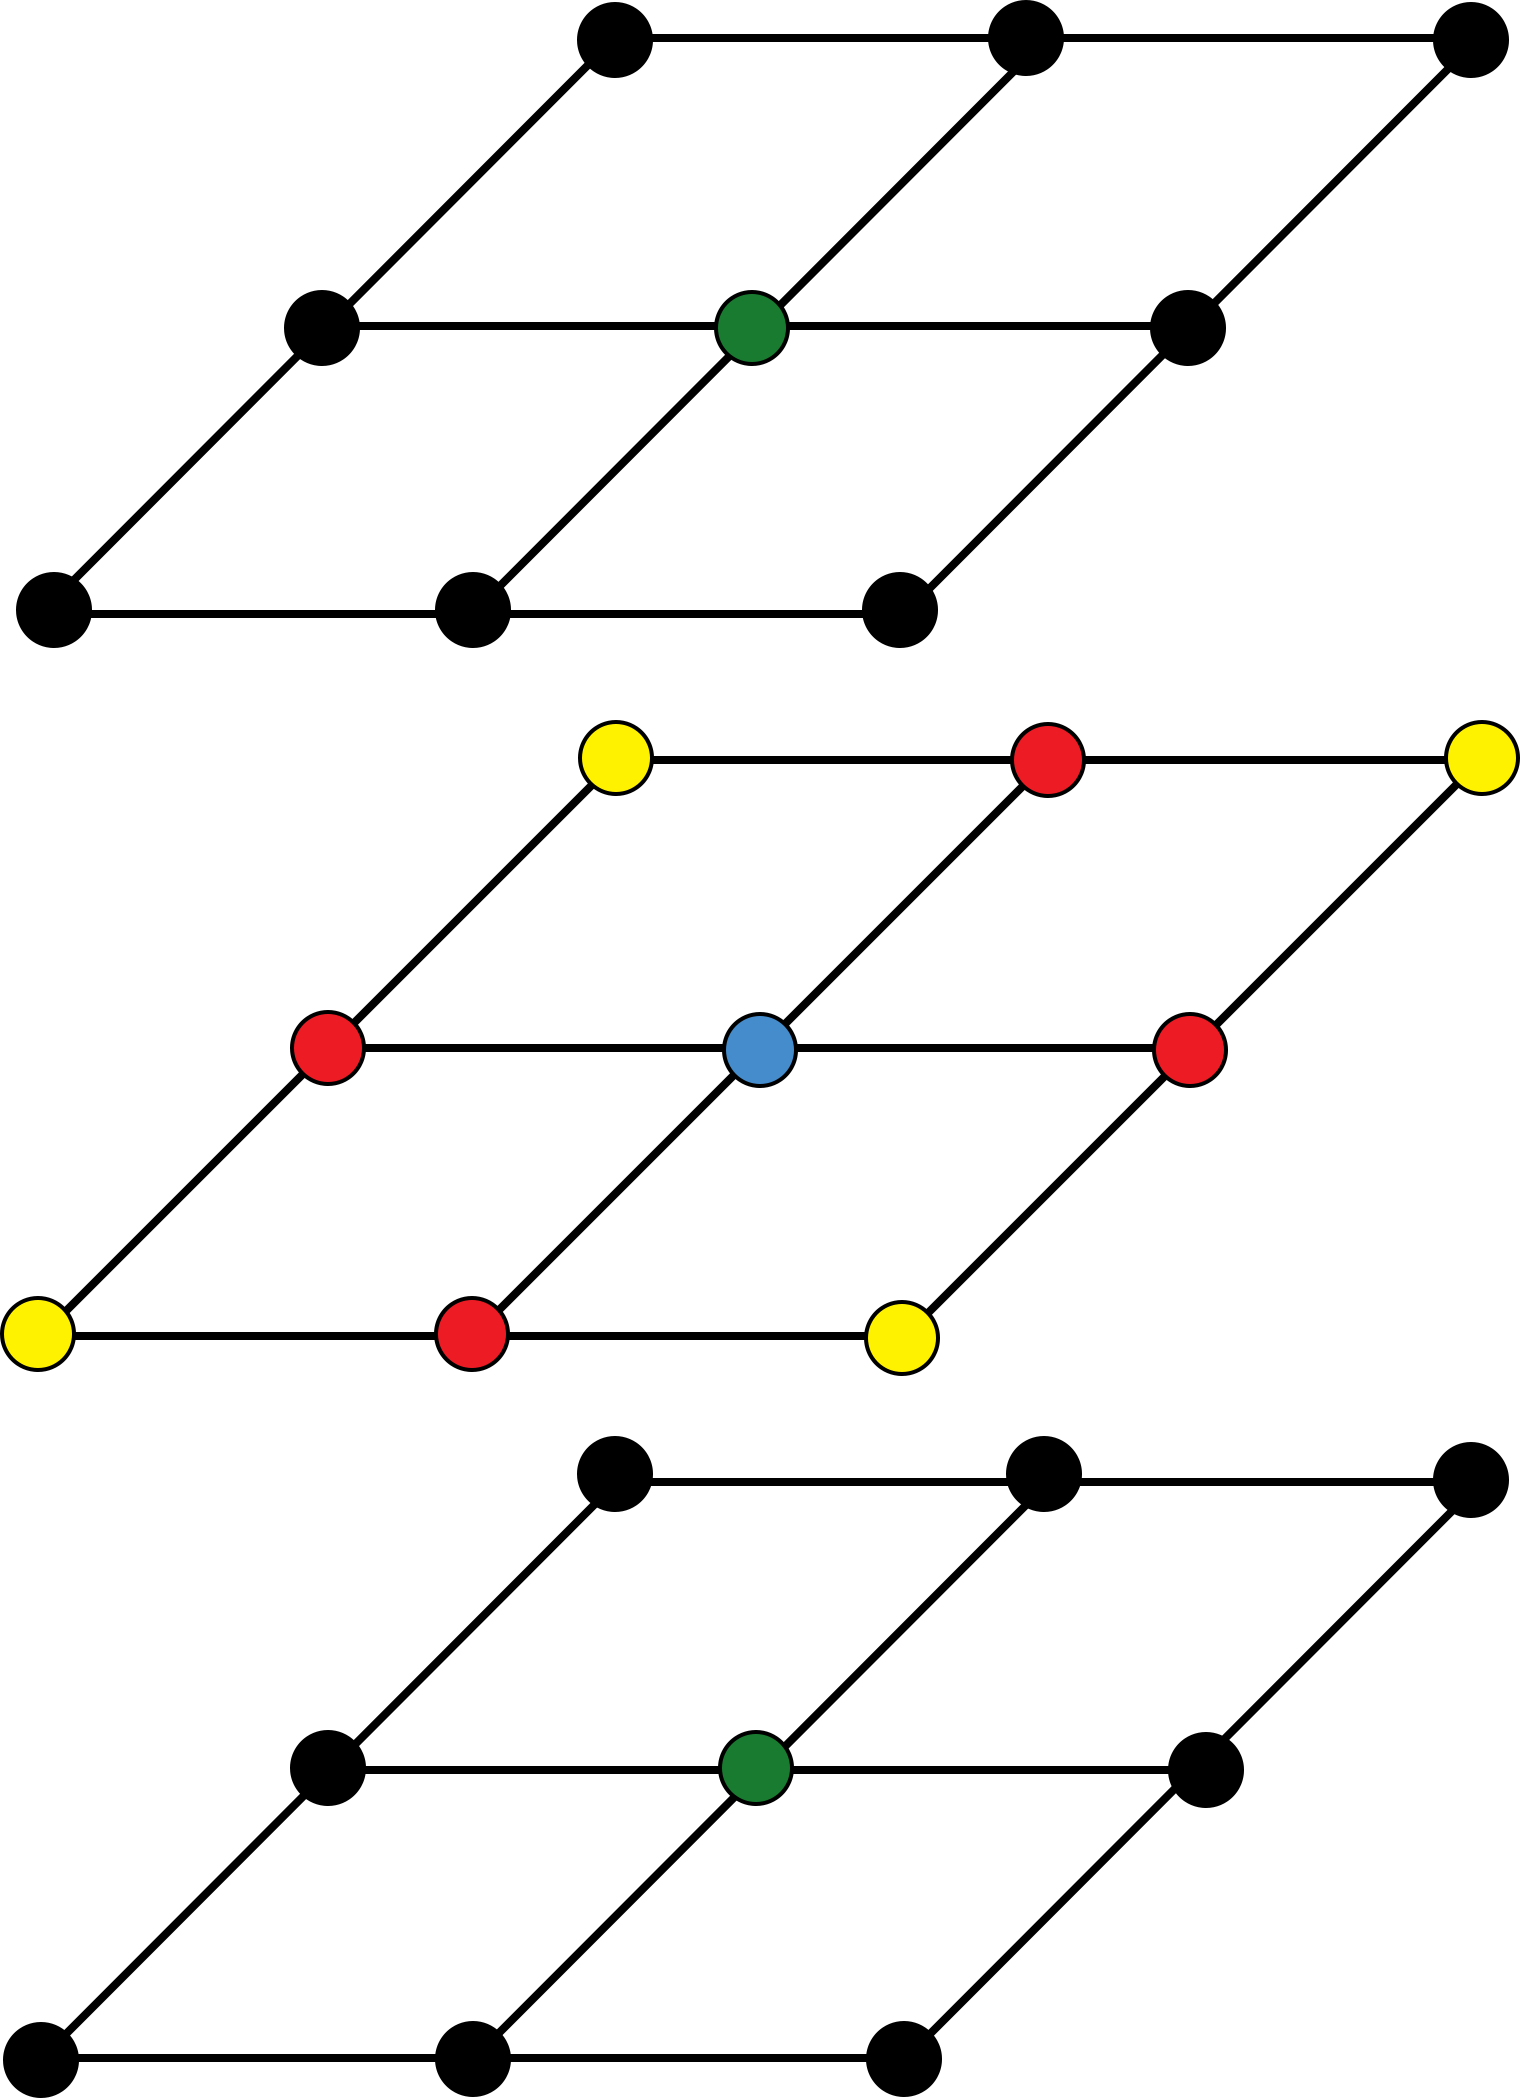
\includegraphics[width=5cm]{BBMG/Face_3D.png}
\centering
\caption{A face centered fine node, shaded blue, surrounded by $4$ coarse nodes, shaded yellow, $4$ dependent nodes, shaded red, $16$ edge nodes that rotates along the coarse nodes and dependent nodes, shaded black, and $2$ free nodes in the center of the coarse cells, shaded green.}
\label{fig:face_center}
\end{figure}
 A face center fine node $i$, Figure~\ref{fig:face_center}, assuming its geometric index is $(x_i,y_i,z_i)$, is adjacent with $4$ nodes that are coincide with a coarse node and $4$ nodes that lie on a coarse cell edge and can be prolongated by the $4$ coarse node within the one ring neighbor hood of $i$. We call them \textit{dependent nodes}. Without loss of generality, let's assume the fine node lies on a xy aligned face. The adjacent coarse node set is then:
 \begin{equation}
 \mathcal{C} = \{(x_i-1,y_i-1,z_i),(x_i-1,y_i+1,z_i),(x_i+1,y_i-1,z_i),(x_i+1,y_i+1,z_i)\}
 \end{equation}
 The set of the dependent nodes that can be prolongated form nodes in $\mathcal{C}$ is then:
  \begin{equation}
 \mathcal{D} = \{(x_i-1,y_i,z_i),(x_i+1,y_i,z_i),(x_i,y_i-1,z_i),(x_i,y_i+1,z_i)\}
 \label{equ:embedding_set}
 \end{equation}
We define the set of fine nodes that is influenced by the rotational DOF of each nodes in $\mathcal{C}$ as:
  \begin{align}
 \mathcal{R}_1 &= \{(x_i-1,y_i-1,z_i-1),(x_i-1,y_i-1,z_i+1)\} \\
 \mathcal{R}_2 &= \{(x_i-1,y_i+1,z_i-1),(x_i-1,y_i+1,z_i+1)\} \\
 \mathcal{R}_3 &= \{(x_i+1,y_i-1,z_i-1),(x_i+1,y_i-1,z_i+1)\} \\
 \mathcal{R}_4 &= \{(x_i+1,y_i+1,z_i-1),(x_i+1,y_i+1,z_i+1)\}
 \end{align}
 Those are the nodes with prescribed displacement in the local problem. With this we can again rearrange the local matrix $\mathbf{L}_i$ similar to equation~\ref{equ:matrix_split}, and compute the prolongation operator similar to equation~\ref{equ:edge_P_2D}.

If define $\mathbf{S^P}_{c,j}$, $j \in \mathcal{D}$ the prolongation stencil, a $3 \times 3$ matrix, from node $j$ to the center node $c$. Similarly, define $\mathbf{S^P}_{j,k}$, $j \in \mathcal{D}$ or $j = c$ and $K \in \mathcal{C}$ the prolongation stencil, a $3 \times 6$ matrix, from coarse node $k$ to a embedded node $j$. The final prolongation stencil from coarse node $k$ to the center node $c$, denoted as $\mathbf{P}_{c,k}$, can therefore be written as:
\begin{equation}
\mathbf{P}_{c,k} = \mathbf{S^P}_{c,k} + \sum_{j \in \mathcal{D}} \mathbf{S^P}_{c,j} \mathbf{S^P}_{j,k}, k \in \mathcal{C}
\end{equation}